\subsection{Как}
\begin{frame}[fragile]{Параллельные алгоритмы}
	\begin{itemize}
		\item Некоторые алгоритмы параллелятся просто:
\begin{minted}{cpp}
int sum = 0;
for (int x : values) sum += x;
\end{minted}
		\item Некоторые "--- естественно и на уровне железа:
\begin{minted}{cpp}
char buf1[100], buf2[100];
fread(file_on_disk1, 1, sizeof buf1, buf1);
fread(file_on_disk2, 1, sizeof buf2, buf2);
\end{minted}
		\item Некоторые не параллелятся:
\begin{minted}{cpp}
int steps = 0;
for (int x = 1; x != 0; x = f(x)); steps++;
\end{minted}
		\item Надо писать специальные алгоритмы для распределённых вычислений.
	\end{itemize}
\end{frame}

\begin{frame}{Иллюстрация}
	\begin{center}
		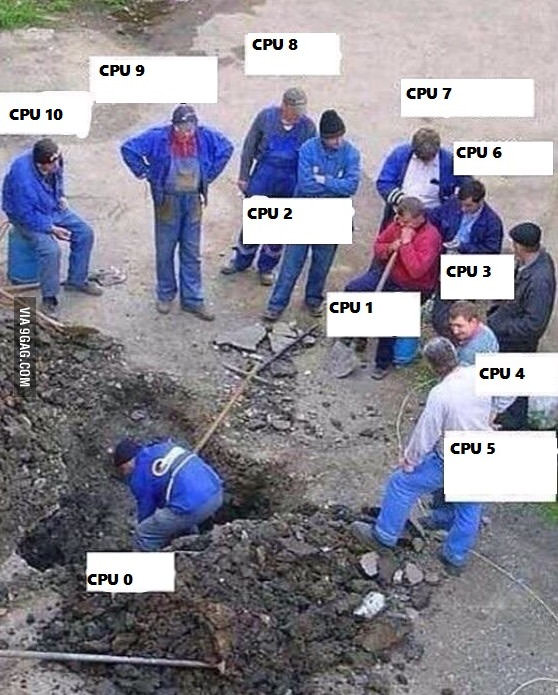
\includegraphics[height=6cm]{cpus-joke.jpg}

		Простое добавление ядер не увеличивает производительность!
	\end{center}
\end{frame}

\begin{frame}{В прикладном хозяйстве}
	\begin{itemize}
		\item Современные ОС различают \textit{потоки} и \textit{процессы}.
		\item Процесс "--- это обычно одно приложение (браузер, IDE, веб-сервер...), у которого может быть много потоков.
		\item Например: у браузера один поток на вкладку; у веб-сервера "--- один поток на клиента.
		\item Изначально у процесса есть только один поток (\textit{главный}), он может создавать другие.
		\item Более строго: процесс "--- это некоторое множество потоков, у которых общая память и другие ресурсы (открытые файлы).
		\item Поток "--- это что-то, выполняющее некий код (есть отдельный стек, свои данные в регистрах процессора, свой код).\
	\end{itemize}
\end{frame}

\begin{frame}{С точки зрения программиста}
	\begin{itemize}
		\item На разных ОС разные методы для работы с процессами или потоками.
		\item Напрямую API уровня ОС, как обычно, никто не использует.
		\item В языке высокого уровня (Java, Python) обычно есть соответствующая библиотека.
		\item Также есть другие классические библиотеки и стандарты:
			\begin{itemize}
				\item pthread "--- Posix Thread, стандарт в C. Будем использовать.
				\item OpenMP "--- высокоуровневое распараллеливание для C/C++/Fortran.
				\item CUDA "--- вычисления на графических картах (ядер тысячи, но они умеют меньше, чем CPU).
			\end{itemize}
	\end{itemize}
\end{frame}

\begin{frame}[fragile]{Типичный псевдокод-1}
\begin{minted}{cpp}
void draw() {
    while (true) {
        wait_for_events();
        process_updates();
        process_mouse_events();
        repaint();
    }
}
int main() {
    Thread draw_thread(draw);
    draw_thread.start();
    // ...
    add_rectangle(10, 10, 30, 40);
    // ...
}
\end{minted}
\end{frame}

\begin{frame}[fragile]{Типичный псевдокод-2}
\begin{minted}{cpp}
void process_client(Client client) {
    string request = client.read();
    string answer = "I've got " + request;
    client.write(answer);
}
int main() {
    while (true) {
        Client client = get_next_client();
        Thread(process_client, client).start();
    }
}
\end{minted}
\end{frame}

\begin{frame}[fragile]{Типичный псевдокод-3}
\begin{minted}{cpp}
void merge_sort(int l, int r) {
    if (l + 1 == r) return;
    Thread t1(merge_sort, l, (l + r) / 2);
    Thread t2(merge_sort, (l + r) / 2, r);
    t1.start(); t2.start(); // Запускаем потоки.
    t1.join(); t2.join();   // Ждём завершения.
    merge(l, r);
}
\end{minted}
\end{frame}
